\chapter{Theory}\label{chapter:theory}

This chapter explains the theoretical concepts needed for understanding the NLP system described in the next chapter. This chapter is broken down into two parts. First part of the chapter explains the terms and terminologies used in Natural Language Processing (NLP) and second part of the chapter explains the concepts  used in Support Vector Machines (SVM).

\section{Natural Language Processing (NLP)}

Natural Language Processing (NLP) is an area of research and application that explores how computers can be used to understand and manipulate natural language text or speech to do useful things \cite{chowdhury2003natural}. The foundations of NLP lie in a number of disciplines, viz. computer and information sciences, formal language theory, linguistics, artificial intelligence, psycho-linguistics,  etc.

\subsection{NLP Basics}\label{sec:NLPPipeline}

NLP systems work on a chunk of text as an input. However, plain text data is unstructured data and all NLP systems preprocess the data in order to convert it into structured representation. There are two types of tasks in NLP, viz. syntactic tasks and semantic tasks \cite{nlpcourse}. All NLP systems work on many of these tasks in order to achieve a certain objective.  

Syntax concerns with proper ordering of the words and its effect on the meaning while semantics deals with literal meaning of the words, phrases and sentences \cite{wiki:sentSeg}. This section presents an overview of syntactic tasks. Most of the NLP systems use syntactic tasks for preprocessing the data.

\subsubsection{Sentence segmentation}

\textit{Sentence segmentation} is the process of dividing a chunk of text into component sentences \cite{wiki:sentSeg}. In English and some other languages, using fullstop ('.') is a reasonable approximation for end of the sentence and can be used to parse the text into sentences. However, the problem is not so trivial due to the use of abbreviations such as "Mr.", "Dr.", etc. For example, in the sentence \textit{"Mr.Smith went to the shops in Jones Street."}, the sentence actually ends after the word \textit{"Street"} and not after abbreviation \textit{"Mr."}. In some languages, the task may become complex since they do not have a proper punctuation character that can be used for approximating sentence boundary.

\subsubsection{Word segmentation}

\textit{Word segmentation} is the process of dividing the text into constituent words \cite{wiki:sentSeg}. Usually, white spaces can be used to parse the text into words in English. Although white spaces are a good approximation for breaking the text into words, sometimes they are not present. For example, the word \textit{couldn't} consists of two words \textit{could} and \textit{not} which cannot be split using a white space. In some other languages like Chinese, words are not separated by spaces.

\subsubsection{Tokenization}

A token is a basic processing unit in NLP system. In most of the cases, a token is a word. However, in some NLP systems, a token can also be a sentence or a paragraph depending on the objective to be achieved.

\subsubsection{Stemming and Lemmatization}

\textit{Stemming} and \textit{lemmatization} are the processes used for reducing a word to a base form. Such reductions are useful for NLP systems. However, there is a difference between \textit{stemming} and \textit{lemmatization}. \textit{Stemming} refers to the crude heuristic process of chopping off the ends of the words in hope of finding the base word \cite{stemminglemmatization}. This works most of the time. For example, the stem of words \textit{running} and \textit{runs} is \textit{run}. \textit{Lemmatization} usually extracts the base word properly with the use of vocabulary and morphological analysis of the words \cite{stemminglemmatization}. For example, the base of \textit{is}, \textit{am} and \textit{are} is \textit{be} which can only be extracted by lemmatization and not by stemming.

\subsubsection{Part of the speech (POS) tagging}

\textit{Part of the speech (POS) tagging} is the process of annotating each word in the sentence with part of the speech tag. This is an important step and is useful for subsequent syntactic parsing and word sense disambiguation \cite{nlpcourse}. 

\subsubsection{Parsing}

There are two views of linguistic structure in NLP, viz., constituency (phrase structure) and dependency structure \cite{parsing}. Both structures are represented as trees. The process of producing these structures correctly is called parsing. There are two types of parsing:

\begin{figure}
\centering
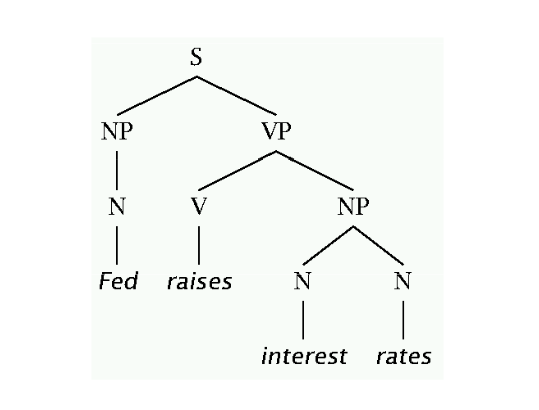
\includegraphics[scale=0.5]{figures/SyntacticParse.png}
\caption{An example of syntactic parsing}\label{fig:SynParse}
\end{figure}

\begin{figure}
\centering
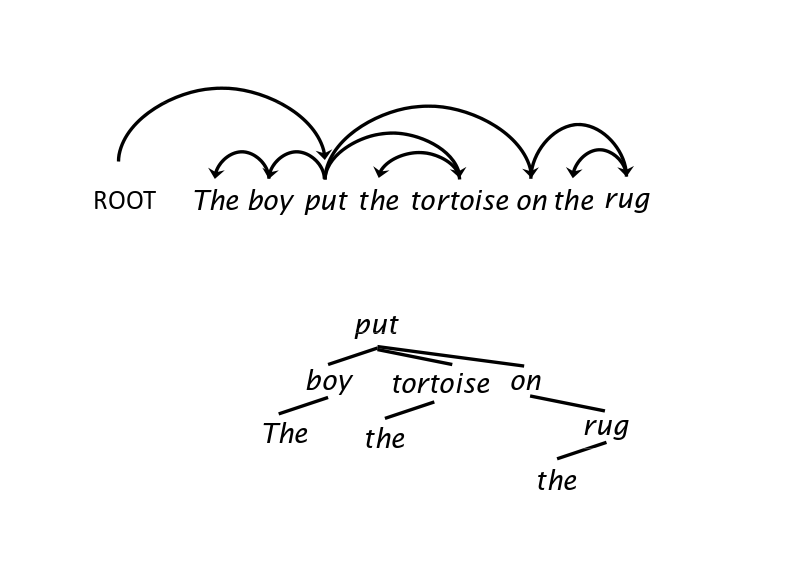
\includegraphics[scale=0.4]{figures/DependencyParse.png}
\caption{An example of dependency parsing}\label{fig:DepParse}
\end{figure}


\begin{itemize}

\item \textit{Syntactic parsing:} The process of producing a constituency structure from a sentence is called syntactic parsing. In constituency structure, the words are organized into phrases which are further organized into a phrase or a sentence. Fig. \ref{fig:SynParse} shows the syntactic parse of sentence \textit{"Fed raises interest rates."}.

\item \textit{Dependency parsing:} The process of producing a dependency parse/structure from a sentence is called dependency parsing. In dependency parsing, the binary relations among the words are used to create a dependency parse tree. In a dependency tree, the words in the sentence act as nodes and the dependency relations between them act as edges. Fig. \ref{fig:DepParse} shows the dependency parse of sentence \textit{"The boy put the tortoise on the rug."}.

\end{itemize}

\subsection{NLP Pipeline}

Most of the NLP systems are actually a complex pipeline of tasks. For any processing to be done, it is necessary to break down the input unstructured text into structured units. Most of the syntactic tasks mentioned in the previous section are used for preprocessing the text. The usual pipeline for any NLP system looks like as shown in the Fig. \ref{fig:NLPPipe}.

\begin{figure}
\centering
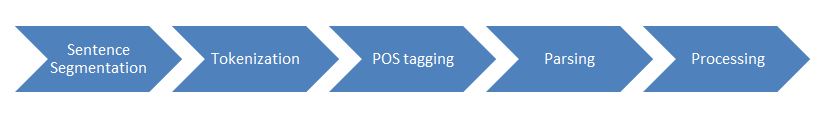
\includegraphics[scale=0.4]{figures/NLPPipeline.png}
\caption{NLP pipeline}\label{fig:NLPPipe}
\end{figure}

\subsection{NLP Semantic tasks}

Semantic tasks in NLP deal with extracting meaningful information from the text. Following are different types of semantic tasks:

\subsubsection{Named Entity Recognition (NER)}

Named entities are atomic elements in the text belonging to predefined categories \cite{ner1} such as the names of the persons, organizations, locations, etc. In simple words, \textit{Named Entity Recognition} is the task of taking unannotated block of text such as \textit{"Jim bought 300 shares of Acme Corp. in 2006."} and converting it into an annotated block like \textit{"$[Jim]_{Person}$ bought 300 shares of $[Acme Corp.]_{Organization}$ in $[2006]_{Time}$."} \cite{wiki:ner}.

\subsubsection{Machine translation}
% Search Engines
% Helping the human translators

\textit{Machine translation} is the process of translating text or speech from one language to another automatically without human intervention.

\subsubsection{Relationship Extraction}\label{sec:RE}
% task of extracting information from emails

\textit{Relationship extraction} is the process of identifying relationship between different named entities present in the sentence. For example, in the sentence \textit{"$TUM_{university}$ is located in $Munich_{location}$"}, \textit{TUM} is a named entity of type \textit{university}, \textit{Munich} is a named entity of type \textit{location} and \textit{TUM} and \textit{Munich} are related by a relation \textit{located-in(TUM,Munich)}.

\subsubsection{Coreference resolution}

\textit{Coreference resolution} is the task of finding all expressions that refer to the same entity in the text. For example, in the sentence \textit{"Sally arrived, but nobody saw her."}, \textit{her} refers to \textit{Sally} in the sentence.

\subsubsection{Other semantic tasks}
% Other tasks: 
% 2. word sense disambiguation 
%4. Question Answering 
%5. Document summarization 
%- summary of an article
%6. Dialog
%- Human machine communication

There are a plethora of other semantic tasks in NLP such as sentiment analysis, spam detection, information extraction, question answering, word sense disambiguation, document summarization, etc.

%TODO write following sections
%\subsection{Relationship Extraction}\label{sec:RE}
% Write that of all the tasks that you can do in NLP, relationship extraction
% is one of them
% Write Examples

%\subsection{Grammatical Dependencies}
%Dependency Parser

\section{Support Vector Machines}\label{sec:SVM}
% Write about some of the theory behind SVM

Machine Learning algorithms are a set of algorithms that can learn from data. Machine learning tasks are broadly classified into supervised learning and unsupervised learning. In supervised learning, the algorithms are given a set of data along with their labels and the goal for algorithms is to learn the rule that maps the input data to their labels. In unsupervised learning, the data is given without labels and the goal for algorithms is to find the hidden pattern.

Support vector machines (SVM) are supervised learning models that can be used for the task of classification and regression. SVM is widely used for the task of classification, i.e., classifying the data into one of the predefined classes/labels.

\subsection{Mathematical formulation}
\begin{figure}
\centering
\begin{minipage}{.5\textwidth}
  \centering
  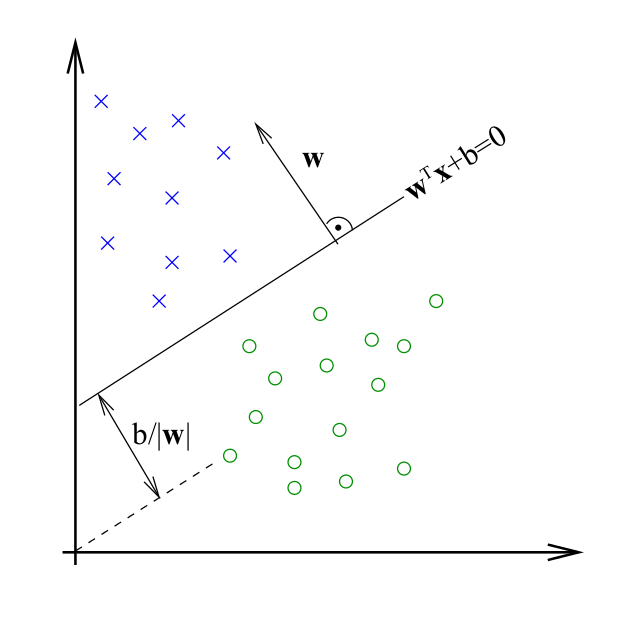
\includegraphics[width=.95\textwidth]{figures/SVMFigure1.png}
  \caption{Data separating hyperplane}
  \label{fig:SVM1}
\end{minipage}%
\begin{minipage}{.5\textwidth}
  \centering
  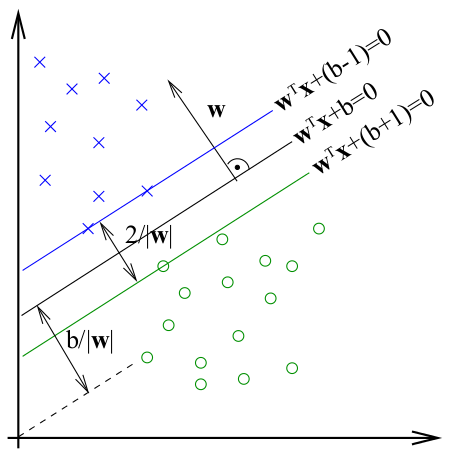
\includegraphics[width=.95\textwidth]{figures/SVMFigure2.png}
  \caption{Maximum margin classifier}
  \label{fig:SVM2}
\end{minipage}
\end{figure}

%\begin{figure}
%\centering
%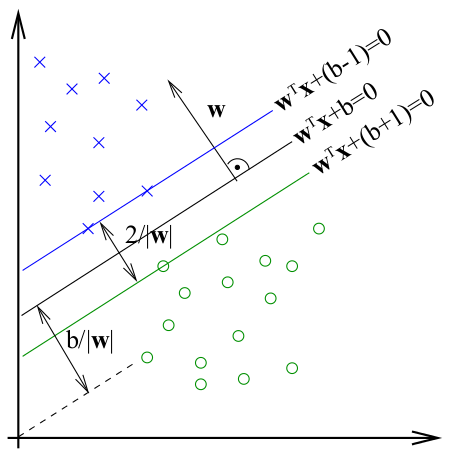
\includegraphics[scale=0.4]{figures/SVMFigure2.png}
%\caption{Maximum margin classifier}\label{fig:SVM2}
%\end{figure}
%
%\begin{figure}
%\centering
%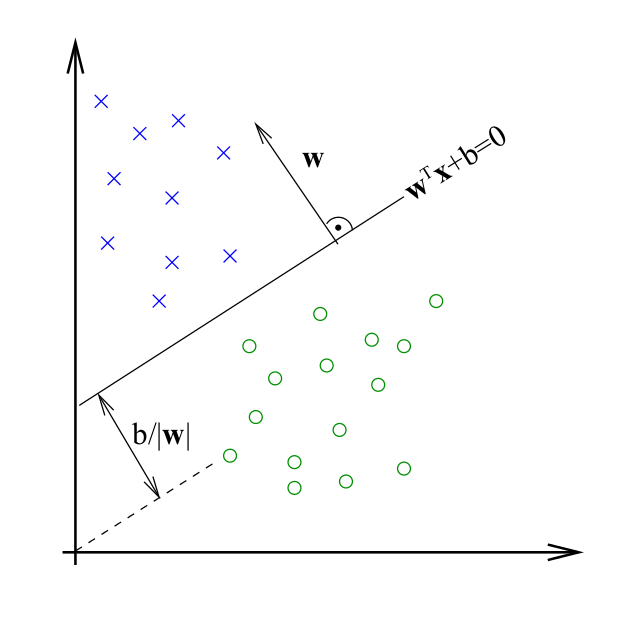
\includegraphics[scale=0.4]{figures/SVMFigure1.png}
%\caption{Hyperplane separating data points}\label{fig:SVM1}
%\end{figure}


SVM tries to build a hyperplane that separates the data points belonging to different categories. For example, as shown in Fig. \ref{fig:SVM1}, the hyperplane separating blue points and green points is given by:

$$
\mathbf{w}^{T}\mathbf{x} + b = 0
$$

where $\mathbf{w}$ is a vector normal to the hyperplane and $\mathbf{x}$ are the set of all points that satisfy above equation and are located on the hyperplane. The projection length from the origin is denoted by $\frac{b}{|\mathbf{w}|}$. 

For a point $\mathbf{x}_1$ having projection length greater than $\frac{b}{|\mathbf{w}|}$, $\mathbf{w}^{T}\mathbf{x}_1 + b > 0$ and the point is classified as a blue point. Similarly, for a point $\mathbf{x}_2$ having projection length less than $\frac{b}{|\mathbf{w}|}$, $\mathbf{w}^{T}\mathbf{x}_2 + b < 0$ and the point is classified as a green point. Therefore, the class of a new point $\mathbf{x}$ is given by:

\begin{align}
\begin{aligned}
%$$
h(\mathbf{x}) = sgn(\mathbf{w}^{T}\mathbf{x} + b) \label{eq:sgn}
%$$
\end{aligned}
\end{align}

Intuitively, the greater the distance of the points on each side of the hyperplane, the better the classification. Therefore, efforts are made to construct a maximum margin classifier.  Such a classifier will make it more likely to classify a new point on the right side of the dividing hyperplane. Hence, the problem of constructing a hyperplane is refined to constructing a hyperplane that separates both classes and has maximum margin.

Figure \ref{fig:SVM2} shows an maximum margin classifier such that the size of the margin is given by:

$$
m=\frac{2}{|\mathbf{w}|}
$$

For such a classifier, if the target classes for data point $x_i$ are given by $y_i \in \left\lbrace -1, +1 \right\rbrace$, then the constraints

\begin{align}
\begin{aligned}
\mathbf{w}^{T}\mathbf{x}_i + b \geq +1 \quad \text{for} \quad y_i = +1 \\
\mathbf{w}^{T}\mathbf{x}_i + b \leq -1 \quad \text{for} \quad y_i = -1
\end{aligned}
\end{align}

can be condensed into 

$$
y_i (\mathbf{w}^{T}\mathbf{x}_i + b) \geq 1 \quad \text{for all} \quad i
$$

Therefore, the problem of finding a maximum margin classifier can be formulated in the form of constrained convex optimization problem as follows:

\begin{align}
\begin{aligned}
\text{minimize} \quad f_0(\mathbf{w},b) &= \frac{1}{2} \mathbf{w}^{T} \mathbf{w} \\
\text{subject to} \quad f_i(\mathbf{w},b) &= y_i (\mathbf{w}^{T}\mathbf{x}_i + b) -1 \geq 0 \quad \text{for} \quad i = 1,...,m
\end{aligned}
\end{align}

Upon solving the optimization problem, the weights are found to be linear combination of training samples:

$$
\mathbf{w} = \sum^{m}_{i=1} \alpha_i y_i x_i
$$

Substituting the weight vector into \ref{eq:sgn}, the class of a new point $\mathbf{x}$ is given by:

$$
h(\mathbf{x}) = sgn(\sum^{m}_{i=1} \alpha_i y_i x_i^{T} x_i + b)
$$

\begin{figure}
\centering
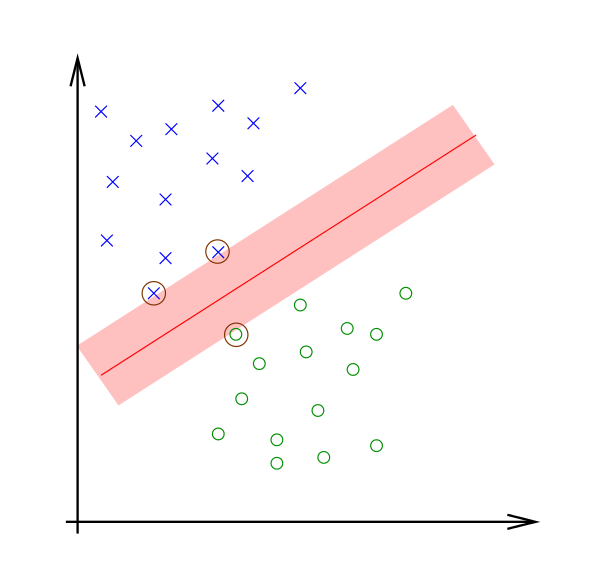
\includegraphics[scale=0.4]{figures/SVMFigure3.png}
\caption{Support vectors}\label{fig:SVM3}
\end{figure}

Actually, only the points lying on the margin contribute to the weight vector and are therefore called support vectors. The support vector points are encircled in the figure \ref{fig:SVM3}. The algorithm derives its name from "support vectors".

\subsection{Regularization parameter} \label{subsec:RegPar}

One of the hyperparameters used in support vector machines is known as regularization parameter and denoted by $\mathbf{C}$. Regularization parameter controls the trade off between achieving a low training error and achieving a low testing error. It tells the SVM optimization how much it should avoid misclassifying each training example. In other words, using large values of $\mathbf{C}$ may fit the training data very well and can result in overfitting. On the other hand, small values of $\mathbf{C}$ may lead to lower performance on training set but better generalization.
